\subsection{Product perspective}

\subsubsection{Further details on shared phenomena}

\paragraph{Report:}
is composed by the picture regarding violation and by its metadata: type, road or GPS coordinates, date-time and so forth.
The report transfer is done via HTTPS, in order to be encrypted since it contains private data.
Once it is received, the algorithm checks the picture trustfulness.

\paragraph{Authority notification:} it has to contain the data of the violation that authorities can use to generate traffic tickets.

\paragraph{Data and statistics visualization:} crossed data about violations and accidents are used to create the map with colored road according to the number of violations.


\begin{center}
	\begin{tabular}{ | l | p{6cm} | } 
		\hline
		PHENOMENA & SHARED  \\ 
		\hline
		User check his profile &   Yes \\
		\hline
		User sends the photo of a violation & Yes \\ 
		\hline
		SafeStreets retrieve licence plate & No \\ 
		\hline
		SafeStreets retrieve position & Yes \\ 
		\hline
		SafeStreets check reliability of the photo & No \\ 
		\hline
		SafeStreets locate the most unsafe area &  No\\ 
		\hline
		SafeStreets provide suggestions & Yes \\
		\hline
	\end{tabular}
\end{center}

\subsubsection{Domain model}

The platform has to manage different entities. Some of them are linked and they shared data and function.
The entities are: 
\begin{itemize}
\item Users
\item Local authorities
\item Reports about possible violations (now defined as Report)
\item Real violations
\item Statistics
\end{itemize}


When the user see a parking violation, he could take a picture of the involved car (is important that the license plate is visible) and sends it to the system with all the relative information about the type of violation and the road.

All of these information are used to create report entities that are analyzed by the platform’s algorithm.

If the report is genuine, these data can be used by authorities to generate traffic tickets, with their systems.

Furthermore, they can analyze which are unsafe areas or the vehicles that commit the most violation.

Results are also available inside SafeStreets.
The same operation is done automatically by the platform, crossing reports from users and accidents information provided by authorities.


\subsubsection{Class diagram}
\begin{figure}[H]
	\centering
	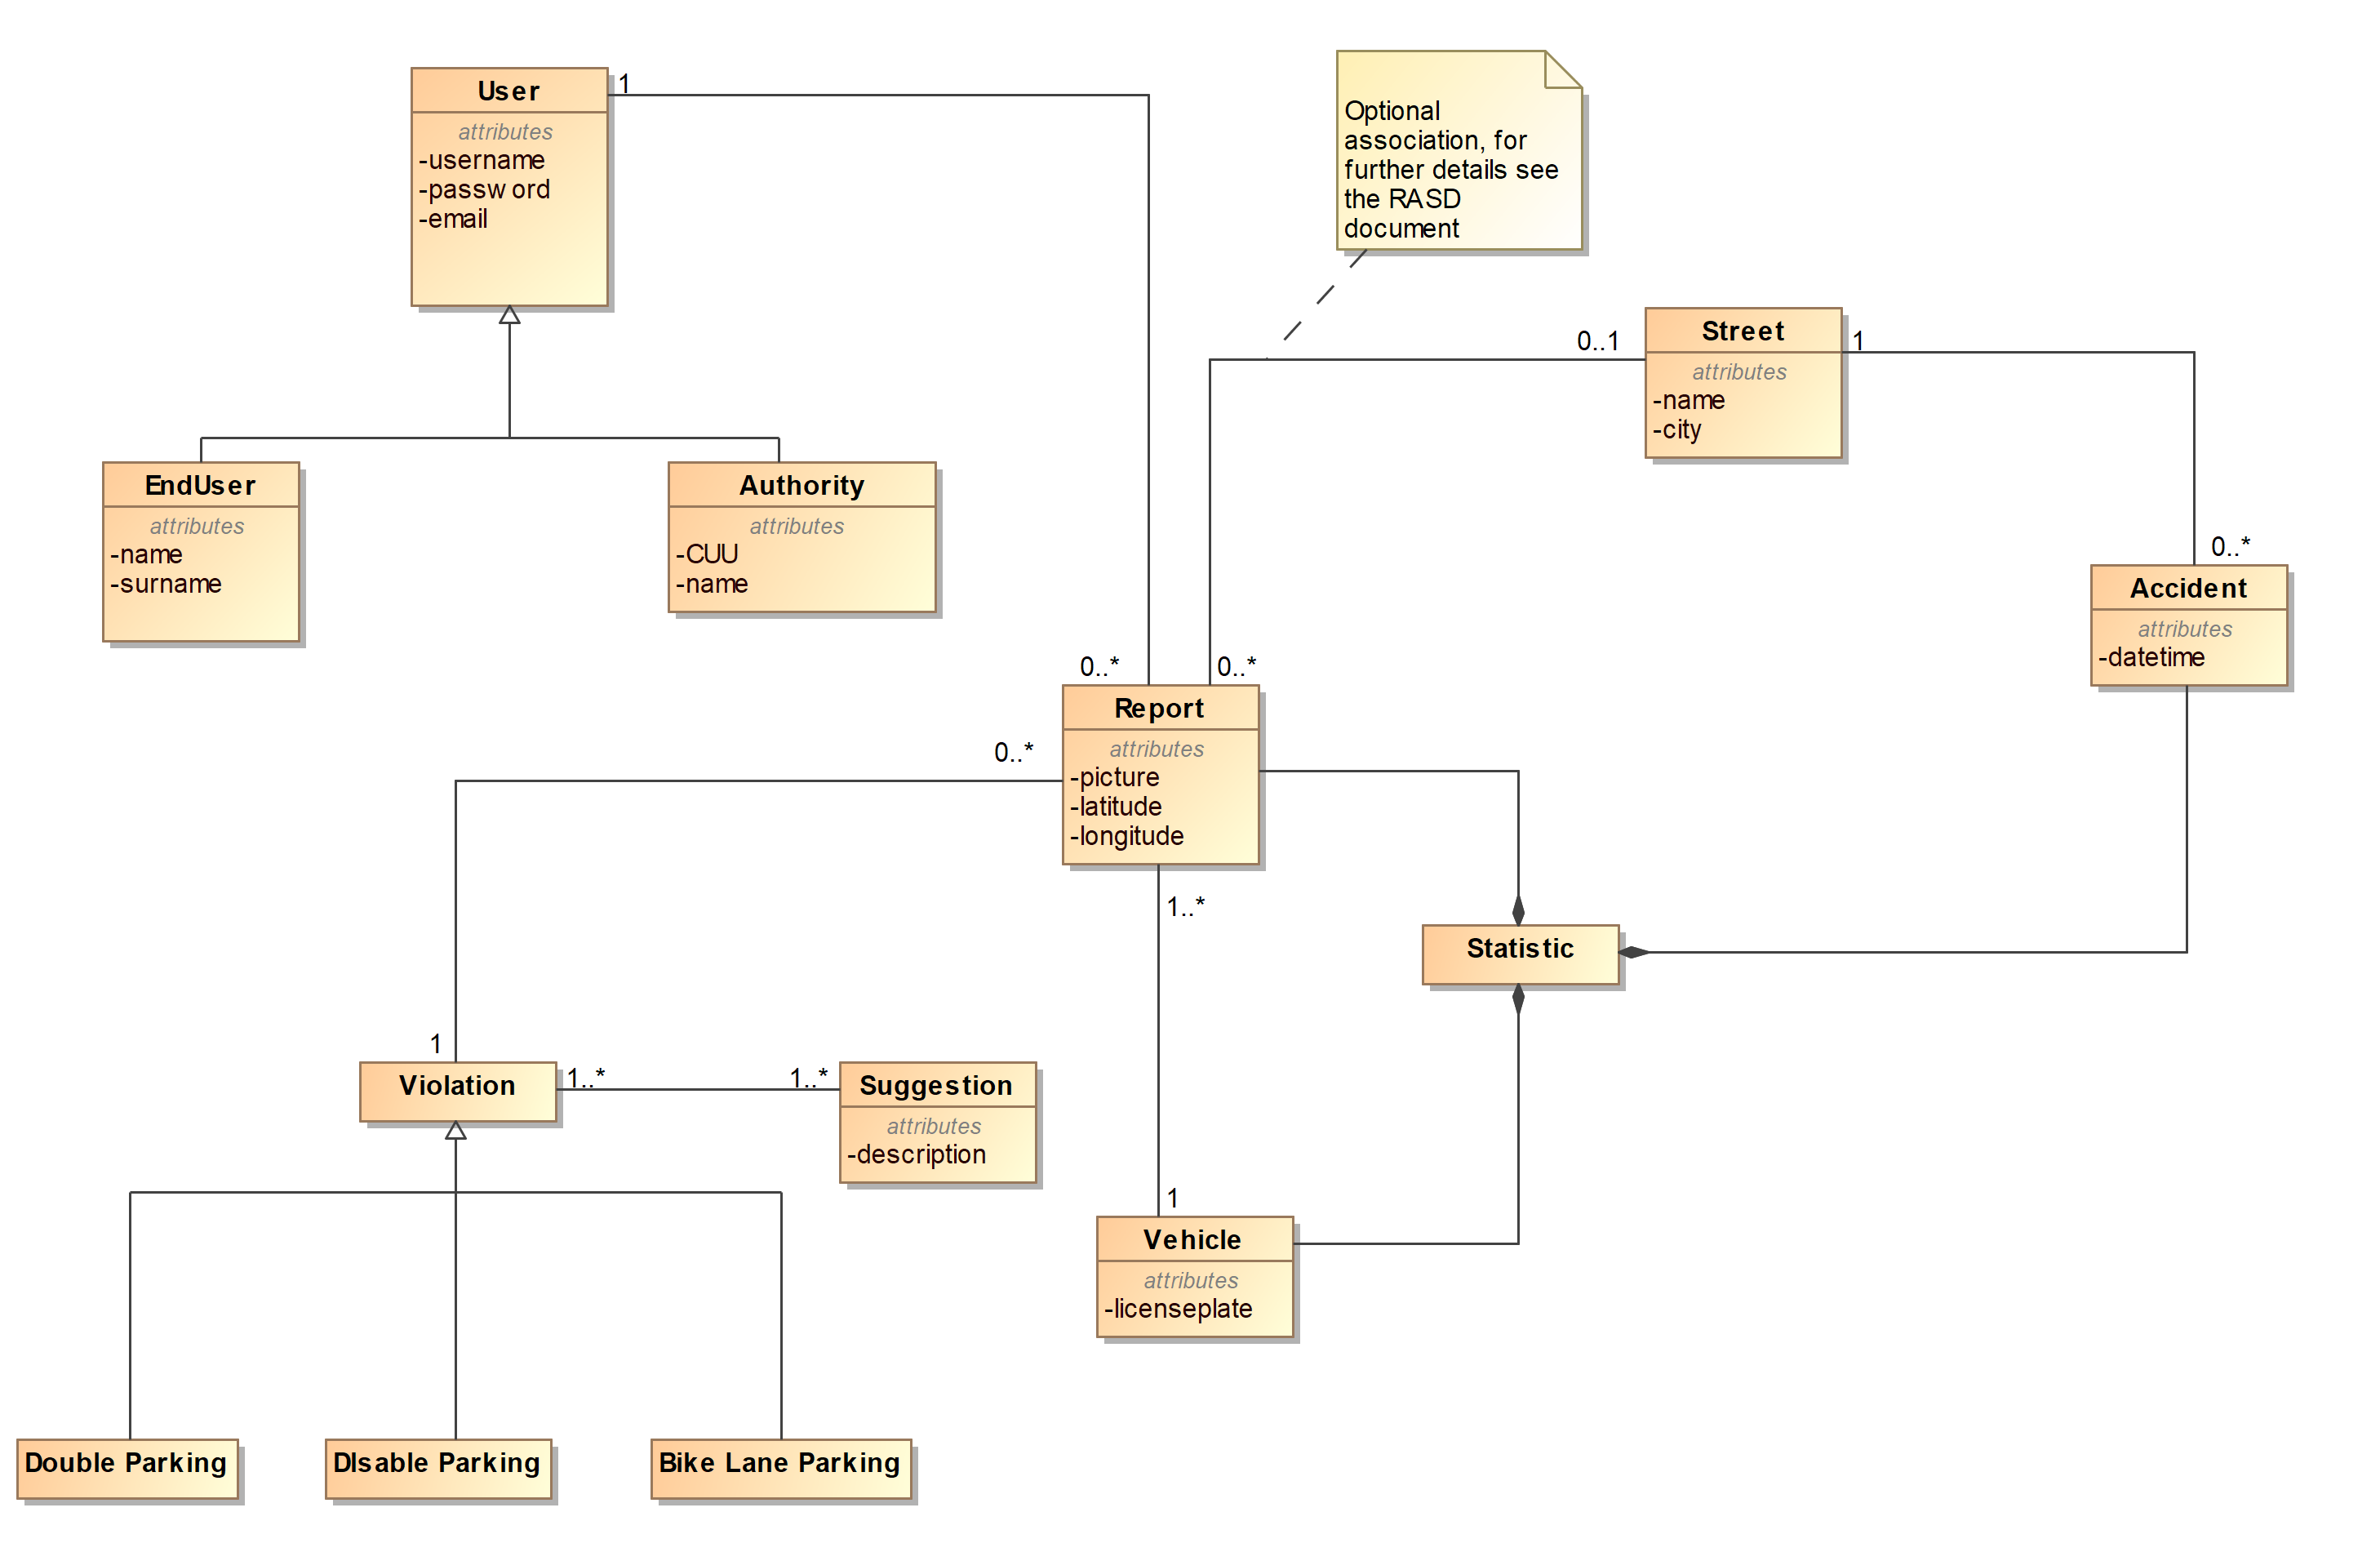
\includegraphics[width=1.12\linewidth]{Images/ClassDiagram.png}
	\caption{Class Diagram}
\end{figure}
The association between Report and Street is optional because we retrieve the position of the report automatically using GPS. Only in case of problem with this operation, we require the address to the user. In this case, SafeStreets calulates the coordinates using the address provided by the user. We use the andress also in case of report made in a place different from the one where the violation occurred. 
\subsubsection{Statechart}
\begin{figure}[H]
	\centering
	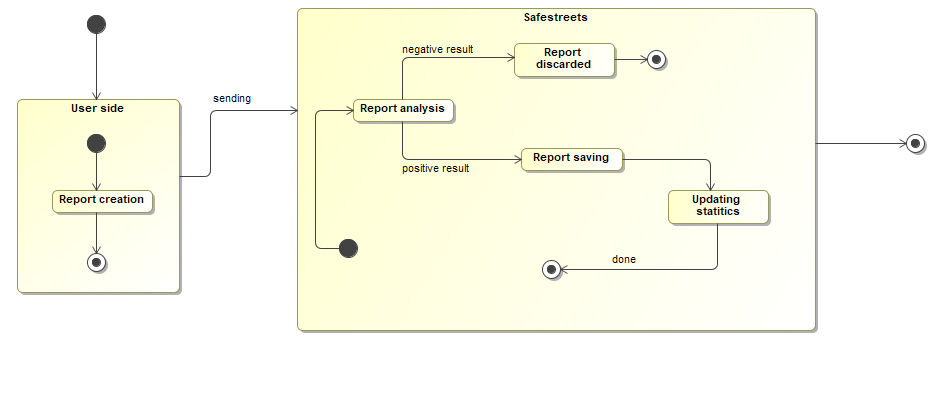
\includegraphics[width=1.12\linewidth]{Images/ReportLifeCycle.png}
	\caption{Report life cycle}
\end{figure}
\begin{figure}[H]
	\centering
	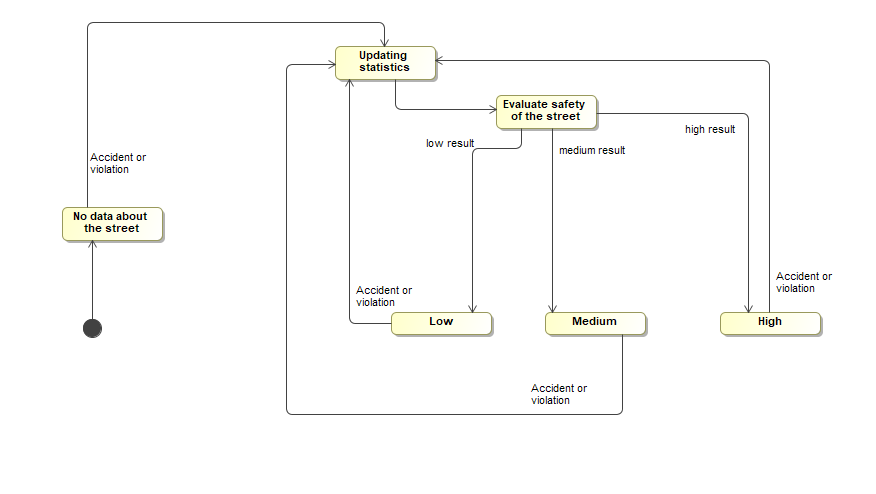
\includegraphics[width=1.12\linewidth]{Images/StreetLifeCycle.png}
	\caption{Street life cycle}
\end{figure}
\newpage

\subsection{Product functions}
Considering the objectives requested by SafeStreets, main functions are described below:

\subsubsection{Notify Traffic Violations RE.1}
The main requirement of the application is to provide users a smart and effortless tool to notify authorities when traffic violations occur.

Users are able to select the type of violation, providing the name of the street, or using their GPS position, and uploading a picture containing the license plate that will be read by an algorithm.

\subsubsection{License Plate Recognition RE.2}
License plate recognition functionality is crucial for SafeStreets, from the license plate we can get information about the owner, the vehicle and its specs.

The fact that there isn't a human being responsible for manually recognizing license plates is important for the scalability, when the application will be used on a large scale.

Automatic number-plate recognition (ANPR) technology consists in seven primary algorithms that the software requires: Plate localization, Plate orientation and sizing, Normalization, Character segmentation, Optical character recognition, Geometrical analysis, Averaging of the recognized values to produce a more reliable or confident result.

Due to the fact that the image will be widely analyzed, it must be in high resolution with no blur and in a good lighting context.

\subsubsection{Data Collection RE.3}
Due to the fact that data is the most valuable asset of modern industry, data collection is important for all statistics, information and data visualization that SafeStreets provides.

It collects data coming from different sources: users inputs, municipality and police databases.
Data collection involve several practices about correctness and security.

\subsubsection{Data Visualization RE.4}
A portion of the application is dedicated to data visualization by showing a map on which the streets/areas are colored according to the frequency of violations and accidents, compared to the average numbers: 
\begin{itemize}
\item red = high
\item yellow = medium
\item green = low
\item white = no data
\end{itemize}

Also there is a part of the UI where authorities can see statistics about vehicles and their violations.

\subsubsection{Data Sets Analysis RE.5}
The functionality of data analysis is crucial for finding patterns in data sets.

\subsubsection{Suggest Possible Interventions RE.6}
Thanks to data sets analysis, SafeStreets can suggest possible interventions for already identified "high-violation" streets.

For each type of violation is assigned one or more possible interventions that will help to decrease the occurrence of that specific violation.


\subsubsection{Information Integrity RE.7}
Data integrity is defined as maintenance and assurance of data consistency over its entire life-cycle.

Ensuring that data are correct and information are never altered is crucial, because local police could take the information about violations coming from SafeStreets.

\subsubsection{Generating Traffic Tickets RE.8}
This functionality is not an internal feature of the application. 

Our scope is to provide the police, data about violations and with this information the municipality could generate traffic tickets with their own systems..

For this reason SafeStreets exposes REST API endpoints to allow authenticated authority users, in this case the police, to get violations information.


\subsection{User characteristics}

The following actors are the users of this application:

\begin{itemize}
	\item End users
\end{itemize}

The end user is a person who, after the sign up, can use SafeStreets to notify traffic violations, consult statistics and see the map with violation information for each street.

\begin{itemize}
	\item Authorities:
	\subitem Municipality
	\subitem Local police
\end{itemize}


Authority is an organization who, after a different sign up from end users, using CUU code, can use SafeStreets to get information about traffic violations for generating traffic tickets, consult possible interventions suggested, see statistics and the map with violation information for each street.
Also they can provide their data to SafeStreets, in this way our platform is able to cross authorities data with its own data.

\subsubsection{Assumptions, dependencies and constraints}
	In this document it is supposed that:
\begin{itemize}
	\item 
	in the country where SafeStreets will be used, the law admits these type of systems.
	
	\item 
	we consider only the following type of violations
	\subitem
	Double parking
	\subitem
	Disable parking
	\subitem
	Bike lane parking
\end{itemize}



